%第4章:システム仕様

本章では,SAS-L2を用いたセキュアな組込みシステムについての仕様を述べる.

\section{SAS-L2を用いたセキュアな組込みシステムの概要}
はじめに,SAS-L2を利用したセキュアな組込みシステムの概要図を図\ref{fig:gaiyo}示す.

\begin{figure}[H]
\begin{center}
	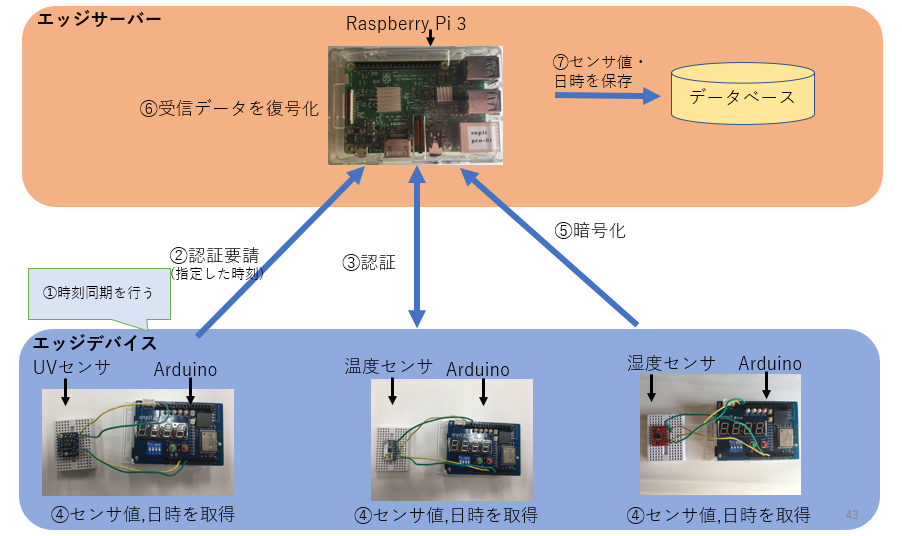
\includegraphics[height=80mm]{gaiyo.png}
	\caption{SAS-L2を利用したセキュアな組込みシステムの概要図}
\label{fig:gaiyo}
\end{center}
\end{figure}

Raspberry Piをエッジサーバーとし,3台のArduinoをエッジデバイスとして利用する.
図\ref{fig:gaiyo}のように,エッジデバイスにはそれぞれ,UVセンサ,温度センサ,湿度センサを接続している.
データベースには,エッジデバイスから収集したデータを保存する.
以降,エッジサーバーをサーバー,エッジデバイスをユーザーと定義する.
図\ref{fig:gaiyo}に沿って,SAS-L2を利用したセキュアな組込みシステムの時刻同期,センシングデータ取得,認証,および暗号化通信の処理の流れを説明する.

\begin{enumerate}
	\item ユーザーを起動し,時刻同期を行う.
	\item ユーザーはサーバーに対して,指定した時刻に認証要請を行う.
	\item サーバーは認証要請を受信し,認証要請を送信したユーザーとのSAS-L2認証を行う.
	\item ユーザーは認証完了後,接続されたセンサからセンシングデータ(センサ値)と,
    センシングデータを取得した日時を取得する.
	\item ユーザーは処理4で取得したデータを暗号化しサーバーへ送信する.
	\item サーバーはユーザーから受信したデータを復号し,センシングデータと日時を取得する.
    \item サーバーは取得した,センシングデータと日時をデータベースに保存する.
    \item 処理4から処理7を10回繰り返す.
    \item 処理2から処理8を繰り返す.
\end{enumerate} 

以上のように,指定した時刻になると認証1回,暗号化通信10回を行うシステムとなる.

\section{要件定義}
SAS-L2を利用したセキュアな組込みシステムの要件定義を述べる.
要件定義には,機能要件と非機能要件がある.
機能要件は,システムで実現すべき機能であり,クライアントから求められる機能のことである.
非機能要件は,機能要件以外の要件であり,主に性能やセキュリティ,環境,制約を指す.
\subsubsection{機能要件}
\begin{enumerate}
	\item 指定した時刻にユーザ―からサーバーにコネクションして認証要請を送信する.
	\item サーバーとユーザー間でSAS-L2による認証を行う.
    \item 認証が成功した場合,サーバーとユーザー間でSAS-L2に基づいた暗号化通信を行う.
    \item 認証が失敗した場合,コネクションを切断してシステム概要で述べた処理1からやり直す.
	\item サーバーは受信データを復号してセンシングデータと日時をデータベースへ保存する.
    \item 暗号化通信終了後,サーバーはコネクションを切断し,ユーザーからの認証要請待ち状態となる.
\end{enumerate} 

\subsubsection{非機能要件}
\begin{enumerate}
    \item 複数のユーザーは同時刻に認証要請を送信するので,一台の認証が終了するまで,その他のユーザーは待機状態になる.
    \item サーバーは認証結果をユーザーに送信する.
    \item サーバーとユーザーは認証結果を表示する.
    \item ユーザーは,シリアルモニタに取得したセンシングデータとセンシングデータの取得日時を表示する.
    \item ユーザーは起動後,1度時刻同期を行う.
    \item サーバーは暗号化通信の際,5秒以上データを受信できなければ,コネクションを切断し,認証要請受信の待機状態となる.
	\item 指定した時刻毎に3つのユーザーとの通信を10秒以内に終わらせる.
    \item サーバーはセンシングデータと取得日時を保存する際に,ユーザーごとのテーブルに分けて保存する.
    \item 1度の認証につき,10回の暗号化通信を行う.
	\item ユーザーで,何らかのエラーが発生した場合,赤LEDを点滅させる.
\end{enumerate} 
